% !TeX document-id = {0be8c18c-9430-4e9a-bdd9-12beadebfebc}
% !TeX TXS-program:bibliography = txs:///biber
\documentclass[11pt]{beamer}
\uselanguage{portuguese}
\languagepath{portuguese}
\deftranslation[to=portuguese]{Theorem}{Teorema}
\deftranslation[to=portuguese]{theorem}{teorema}
\deftranslation[to=portuguese]{Example}{Exemplo}
\deftranslation[to=portuguese]{example}{exemplo}
\deftranslation[to=portuguese]{Lemma}{Lema}
\deftranslation[to=portuguese]{lemma}{Lema}
\deftranslation[to=portuguese]{Corollary}{Corolário}
\deftranslation[to=portuguese]{corollary}{corolário}
%\deftranslation[to=portuguese]{and}{e}

\usepackage[brazilian]{babel}
\usepackage[utf8]{inputenc}
\usepackage[T1]{fontenc}
\usepackage{lmodern}
\usepackage{amsmath}
\usepackage{amssymb}
\usepackage{mathtools}
\usepackage{color}
\usepackage{pgfplots}
\usepackage{tikz}
\usepackage{subcaption}
%\usepackage{appendixnumberbeamer}

\newenvironment{transitionframe}{
	\setbeamercolor{background canvas}{bg=yellow}
	\begin{frame}}{
	\end{frame}
}
\usetheme{default}
\usefonttheme{structuresmallcapsserif}

%% I use a beige off white for my background
\definecolor{MyBackground}{RGB}{255,253,218}
\useinnertheme[shadow]{rounded}
\setbeamercolor{block title}{bg=MyBackground}
\setbeamercolor{block body}{bg=MyBackground}
\setbeamercolor{example title}{bg=MyBackground}
\setbeamercolor{example body}{bg=MyBackground}


\newcommand{\blue}[1]{\textcolor{blue}{#1}}
\newcommand{\red}[1]{\textcolor{red}{#1}}
\newcommand{\purple}[1]{\textcolor{purple}{#1}}
\newcommand{\gray}[1]{\textcolor{gray}{#1}}
\setbeamertemplate{navigation symbols}{}
%\setbeamertemplate{page number in head/foot}[appendixframenumber]

%\usepackage{graphics}
\usepackage{graphicx}

\definecolor{blue_emph}{RGB}{0,114,178}
\definecolor{red}{RGB}{213,94,0}
\definecolor{yellow}{RGB}{240,228,66}
\definecolor{green}{RGB}{0,158,115}
\definecolor{purple}{RGB}{204,121,167}
\definecolor{orange}{RGB}{230,159,0}
\definecolor{lightblue}{RGB}{86,180,233}

%\setbeamercolor{frametitle}{fg=blue}
%\setbeamercolor{title}{fg=blue}
\setbeamertemplate{footline}[frame number]
\setbeamertemplate{navigation symbols}{} 
\setbeamertemplate{itemize items}{-}
%\setbeamercolor{itemize item}{fg=blue}
%\setbeamercolor{itemize subitem}{fg=blue}
\setbeamertemplate{enumerate items}[default]
%\setbeamercolor{enumerate subitem}{fg=blue}
\setbeamercolor{button}{bg=MyBackground,fg=blue}
\usefonttheme{structuresmallcapsserif}

%\setbeamercolor{section in toc}{fg=blue}
%\setbeamercolor{subsection in toc}{fg=red}
\setbeamersize{text margin left=1em,text margin right=1em} 


\usepackage{appendixnumberbeamer}

\usepackage[
backend=biber,
style=authoryear,
natbib=true
]{biblatex}
\addbibresource{../bibliography.bib}

\newenvironment{wideitemize}{\itemize\addtolength{\itemsep}{10pt}}{\enditemize}
\newenvironment{wideenumerate}{\enumerate\addtolength{\itemsep}{10pt}}{\endenumerate}
\newenvironment{halfwideitemize}{\itemize\addtolength{\itemsep}{0.5em}}{\enditemize}
\newenvironment{halfwideenumerate}{\enumerate\addtolength{\itemsep}{0.5em}}{\endenumerate}


\author{Luis A. F. Alvarez}
\title{EAE1223: Econometria III}
\subtitle{Aula 5 - Metodologia de Box-Jenkins}
%\logo{}
%\institute{}
\date{\today}
%\subject{}
%\setbeamercovered{transparent}

\begin{document}

\begin{frame}[plain]
	\maketitle
\end{frame}

\begin{frame}{A metodologia}
	\begin{halfwideitemize}
		\item A metodologia de Box-Jenkins consiste numa série de etapas para estimar um modelo {\color{blue}univariado} de {\color{blue}previsão}.
		\begin{halfwideitemize}
			\item Ideia é estimar um modelo simples, embora flexível, aos dados.
		
		\end{halfwideitemize}
	\item Trata-se da metodologia básica de previsão em séries de tempo. 
\begin{halfwideitemize}
	\item Diversas metodologias modernas incorporam o ``espírito'' de Box-Jenkins.
	\item \textit{Benchmark} para avaliar outros modelos de previsão.
\end{halfwideitemize}
	\end{halfwideitemize}
\end{frame}

\begin{frame}{Etapas da metodologia}
	\begin{halfwideitemize}
			\item A metodologia consiste de quatro etapas:
	\begin{halfwideenumerate}
		\item {\color{blue}Identificação}: nessa etapa, avaliamos os dados e identificamos quais modelos são candidatos plausíveis para reproduzir os dados.
		\item {\color{blue} Estimação}: nessa etapa, estimamos os modelos candidatos.
		\item {\color{blue} Diagnóstico:} nessa etapa, avaliamos quais dos modelos se saíram melhor, de acordo com alguns critérios.
		\item {\color{blue} Previsão:} por fim, realizamos a previsão de acordo com nosso modelo.
	\end{halfwideenumerate}
	\item Nesta aula, discutiremos cada uma dessas etapas.
	\item Começaremos revisando a classe de modelos estudadas na metodologia de Box-Jenkins.
\end{halfwideitemize}
\end{frame}




\begin{transitionframe}
	\begin{center}
		{\Huge   Modelos considerados}
	\end{center}
\end{transitionframe}

\begin{frame}{MA(q)}
	\begin{halfwideitemize}
		\item Dizemos que uma série de tempo $\{Y_t\}$ segue um MA(q) se:
		\begin{equation*}
			Y_t =\alpha + \epsilon_t + \sum_{j=1}^q \theta_j \epsilon_{t-j} 
		\end{equation*} 
		onde $\{\epsilon_t\}$ é um ruído branco.
		\item Série hoje depende diretamente da realização atual e das últimas $q$ realizações de um ruído branco.
		\item \textbf{Todo} processo de média móvel é fracamente estacionário.
		\begin{halfwideitemize}
			\item De fato, $\mathbb{E}[Y_t] = \alpha$, $\mathbb{V}[Y_t] =\left(1+\sum_{j=1}^q \theta_j^2\right) \sigma^2_\epsilon$, $\text{cov}(Y_t, Y_{t-s})= (\theta_s +\sum_{j=s+1}^q \theta_j \theta_{j-s})\sigma^2_\epsilon$ se $s\leq q$ e $0$ do contrário. Correlação morre após $q$ períodos.
		\end{halfwideitemize}
		\item Um processo MA(q) é dito \textbf{invertível} se pode ser escrito como:
		\begin{equation*}
			Y_t = \omega + \sum_{j=1}^\infty \psi_j Y_{t-j} + \epsilon_t
		\end{equation*}
		(MA(q) pode ser representado como AR($\infty$)).
	\end{halfwideitemize}
\end{frame}
\begin{frame}{AR(p) estacionário}
	\begin{halfwideitemize}
		\item Dizemos que uma série de tempo $\{Y_t\}$ segue um AR(p) estacionário se ela se escreve como:
		\begin{equation*}
			Y_t =\alpha + \sum_{j=1}^p \beta_j Y_{t-j} + \epsilon_t
		\end{equation*} 
		onde $\{\epsilon_t\}$ é um ruído branco e os coeficientes $\beta_j$ são tais que o processo resultante é fracamente estacionário.
		\item Série hoje depende diretamente das realizações passadas nos últimos $p$ períodos, mais um ruído branco.
		\begin{halfwideitemize}
			\item Mas persistência não é tão grande, de modo que a série é estacionária (não há raiz unitária).
		\end{halfwideitemize}
		\item Recorde-se que um AR(p) é estacionário se, e somente se, ele se escreve como um MA($\infty$):
		\begin{equation*}
			Y_t = \kappa + \epsilon_{t} +\sum_{j=1}^\infty \tau_j \epsilon_{t-j} 
		\end{equation*}
	\end{halfwideitemize}
\end{frame}



\begin{frame}{ARMA(p,q) estacionário}
	\begin{halfwideitemize}
		\item Dizemos que uma série de tempo $\{Y_t\}$ segue um ARMA(p,q) estacionário se:
		\begin{equation*}
			Y_t =\alpha + \sum_{i=1}^p \beta_i Y_{t-i} + \epsilon_t + \sum_{j=1}^q \theta_j \epsilon_{t-j} 
		\end{equation*} 
		onde $\{\epsilon_t\}$ é um ruído branco, e os $\beta_i$ são tais que o processo resultante é estacionário.
		\item Combinação dos dois modelos anteriores.
		\item {\color{blue} Metodologia de Box-Jenkins visará a estimar modelos na classe ARMA(p,q).}
	\end{halfwideitemize}
\end{frame}

\begin{frame}{E se os dados forem não estacionários?}
	\begin{halfwideitemize}
		\item Até agora, discutimos a modelagem supondo as séries estacionárias.
		\begin{halfwideitemize}
			\item Como fazer a previsão em casos não estacionários?
		\end{halfwideitemize}
		\item Se as séries apresentarem uma tendência estocástica, trabalhamos com os dados em primeira diferença $\{\Delta y_t\}$. 
		
		\item Conduzidas as etapas da metodologia Box-Jenkins com os dados diferenciados, e encontradas projeções para $\Delta y_t$ fora da amostra, recompomos as projeções  em nível usando o fato de que $y_{t+1} = y_t + \Delta y_{t+1}$.
		\begin{halfwideitemize}
			\item Isto é, se temos $T$ observações, projetamos $\widehat{y_{T+1}} = y_t + \widehat{{\Delta y_{T+1}}}$,  $y_{t+2} = y_t + \widehat{\Delta y_{t+1}} + \widehat{\Delta y_{t+2}}$, e assim por diante.
		\end{halfwideitemize}
		\end{halfwideitemize}
\end{frame}
\begin{frame}{Modelos ARIMA(p,d,q)}
	\begin{halfwideitemize}
				\item Em outras palavras, no caso de raiz unitária, a metodologia irá estimar um modelo {\color{blue}ARIMA(p,1,q)}, da forma:
		\begin{equation*}
			\Delta y_t =\alpha + \sum_{i=1}^p \beta_i \Delta y_{t-i} + \epsilon_t + \sum_{j=1}^q \theta_j \epsilon_{t-j}
		\end{equation*}
		\item De modo geral, se a série é I(d), a modelagem considerará modelos {\color{blue}ARIMA(p,d,q)}:
		$$\Phi(L)(1-L)^d y_t =  \alpha + \Psi(L)\epsilon_t \, ,$$
		para polinômios $\Phi(L)$ e $\Psi(L)$ de grau $p$ e $q$, respectivamente.

	\end{halfwideitemize}
\end{frame}
\begin{frame}{Previsão com tendência determinística}
	\begin{halfwideitemize}
				\item Se séries apresentam tendência determinística, conduzimos a metodologia com dados \textit{detrended}. Calculadas as projeções \textit{detrended}, recompomos projeções em nível usando a tendência estimada.
				
				\item Por exemplo, se estimamos uma tendência linear:
				$$y_t = \tilde{a} + \tilde{b}t + \tilde{\xi}_t$$
				e ajustamos um modelo ARMA  para $\tilde{\xi}_t$, a projeção para fora da amostra é:
				
				$$\widehat{y_{T+h}} = \tilde{a} + \tilde{b}(T+h) + \widehat{\tilde{\xi}_{T+h}}\, ,$$
				onde $\widehat{\tilde{\xi}_{T+h}}$ é a projeção do ARMA para $T+h$ (veremos como calculá-la na etapa de previsão).
	\item Estimação de ARMA para dado \textit{detrended} é equivalente a estimar um modelo ARMA(p,q) com tendência determinística.
$$\Phi(L) y_t =  \alpha + \gamma t + \Psi(L)\epsilon_t \, .$$
	\end{halfwideitemize}
\end{frame}

\begin{frame}{``Filosofia'' da metodologia de Box-Jenkins}
	\begin{halfwideitemize}
		\item A restrição a modelos ARMA(p,q) pode ser entendida a partir do {\color{blue}teorema de decomposição de Wold.}
		\item Segundo esse teorema, \textbf{qualquer processo fracamente estacionário} pode ser representado pela soma de um MA($\infty$), acrescido de uma função determinística dos $y$ no passados:
		$$y_t = \epsilon_t  +\sum_{l=0}^\infty \psi_l \epsilon_{t-l} + \kappa_t \, ,$$
		onde $\kappa_t$ é função ``aproximadamente'' linear de $y_{t{\color{red}-1}}$, $y_{t-2}$\ldots 
			\item Ideia de Box-Jenkins é aproximar essa representação por um ARMA(p,q), com \textit{p} e \textit{q} {\color{blue}pequenos}.
		\begin{halfwideitemize}
			\item Ideia é que aproximação {\color{blue}parcimoniosa}, por ser menos ruidosa, tende a funcionar melhor que modelos muito complexos.
		\end{halfwideitemize}	
	\end{halfwideitemize}
\end{frame}

\begin{transitionframe}
	\begin{center}
		{\Huge   Identificação}
	\end{center}
\end{transitionframe}

\begin{frame}{Identificação de um ARMA(p,q)}
	\begin{wideitemize}
		\item A etapa de identificação da metodologia Box-Jenkins consiste em encontrar quais modelos da classe ARMA(p,q) melhor caracterizam a série de interesse.
		\item A identificação consiste em analisar a função de autocorrelação (FAC) e a função de autocorrelação parcial (FACP) da série estacionária.

	
		
	\end{wideitemize}
\end{frame}

\begin{frame}{Função de autocorrelação serial (FAC)}
	\begin{halfwideitemize}
					\item A {\color{blue}função de autocorrelação (FAC)} de uma série $\{Y_t\}_t$ estacionária é o mapa que associa, a cada número $k > 0$, a autocorrelação de ordem $k$, i.e. $\gamma_k = \text{cor}(Y_t, Y_{t-k})$.
					\item Note que essa função está bem definida para processos estacionários, visto que $\text{cor}(Y_t, Y_{t-k})$ não depende de $t$.
					
					$$\operatorname{cor}(Y_t,Y_{t-k}) = \frac{\operatorname{cov}(Y_t, Y_{t-k})}{\operatorname{sd}(Y_t)\operatorname{sd}(Y_{t-k})} = \frac{\operatorname{cov}(Y_t, Y_{t-k})}{\mathbb{V}(Y_t)}$$
				\end{halfwideitemize}
\end{frame}

\begin{frame}{Função de autocorrelação serial parcial (FACP)}
	\begin{halfwideitemize}
		\item A {\color{blue}função de autocorrelação parcial (FACP)} de uma série $\{Y_t\}_t$ estacionária é o mapa que associa, a cada número $k > 0$, a correlação $\theta_k$ entre $Y_{t}$ e $Y_{t-k}$, {\color{blue}controlando por $Y_{t-1}, Y_{t-2}, \ldots Y_{t-k+1}$}.

	
		

	
		\item A autocorrelação parcial de ordem $k$ ($\theta_k$) é dada pelo coeficente $\tau_k$ associado a $Y_{t-k}$ no modelo preditivo linear:
	\begin{equation}
		\label{pred_model}
		\begin{aligned}
			Y_t = \tau_0 + \tau_1 Y_{t-1} + \tau_2 Y_{t-2} \ldots + \tau_k Y_{t-k} + \nu_t \\
			\mathbb{E}[\nu_t] = 0, \mathbb{E}[\nu_t Y_{t-j}] = 0,\quad j=1,\ldots k
		\end{aligned}
	\end{equation}
	\item Note que função está bem definida para processos estacionários, visto que coeficientes do melhor preditor linear em \eqref{pred_model} não dependem de $t$.
		\end{halfwideitemize}
\end{frame}
\begin{frame}{FAC e FACP estimadas}
	\begin{halfwideitemize}
		\item Na prática, não observamos a FAC nem a FACP de um processo, mas podemos estimá-las usando as realizações da série de interesse.
		\begin{halfwideitemize}
			\item Estimamos a FAC calculando as autocorrelações nos dados.
			
			$$\hat{\gamma}_k = \frac{\sum_{t=1}^{T-k} (y_{t}-\bar{y})(y_{t+k}-\bar{y})}{\sum_{t=1}^{T}(y_t-\bar{y})^2} \, ,$$
			onde $\bar{y} = T^{-1}\sum_{t=1}^T y_t$.
			\item Estimamos a FACP ajustando o modelo \eqref{pred_model} aos dados.
		\end{halfwideitemize}
	
	\end{halfwideitemize}
\end{frame}

\begin{frame}{Inferência sobre FAC e FACP populacionais}
	\begin{halfwideitemize}
				\item Como observamos apenas algumas realizações do processo, gostaríamos de testar hipóteses sobre a FAC e FACP populacionais.
		\item Sob algumas condições mais estringentes, o intervalo $[-2/\sqrt{T}, 2/\sqrt{T}]$ é uma região de aceitação aproximadamente válida para o teste da nula $\gamma_k=0$ ($\theta_k =0$ na FACP)  contra a alternativa bilateral ao nível de significância de 5\%.
		\begin{halfwideitemize}
			\item São esses intervalos que são apresentados, no R, quando computamos a FAC e FACP.
			\item Para autocorrelações (parciais) estimadas que excedem esses limites, rejeitamos a hipótese nula de não autocorrelação (parcial) a essa ordem.
		\end{halfwideitemize}
	
	\end{halfwideitemize}

\end{frame}
\begin{frame}{FAC e FACP amostrais de $\Delta \text{Desemprego}$}
	\begin{figure}
		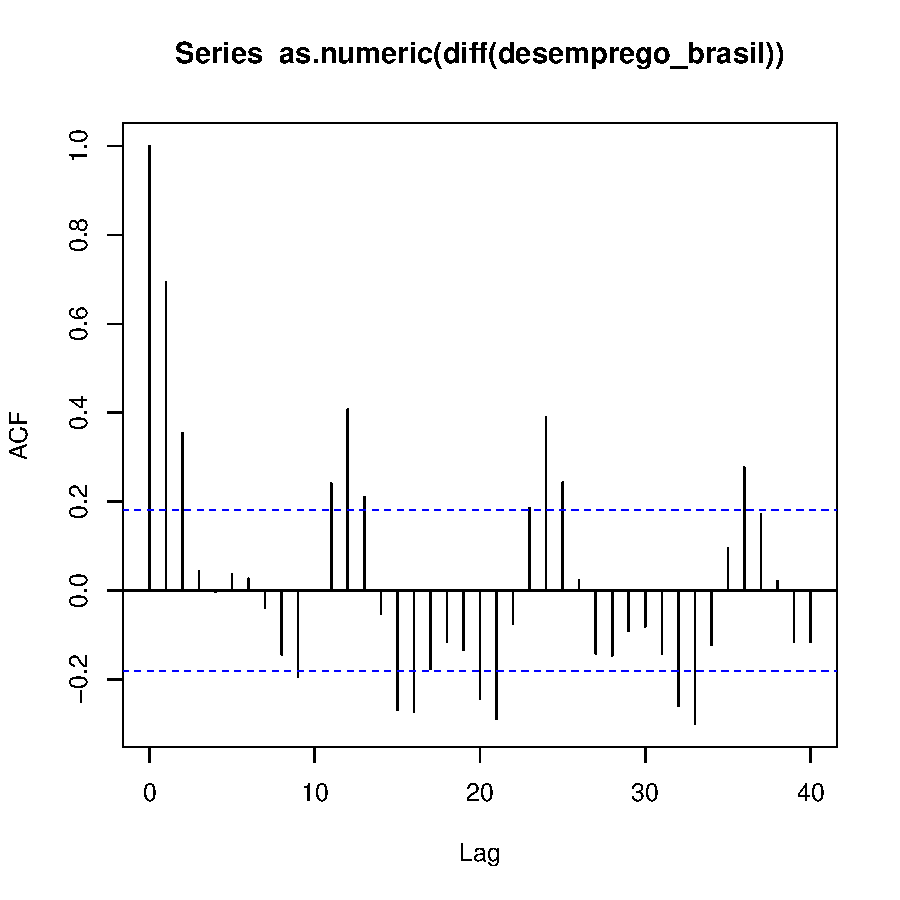
\includegraphics[scale=0.39]{graficos/acf_unemp.pdf} 		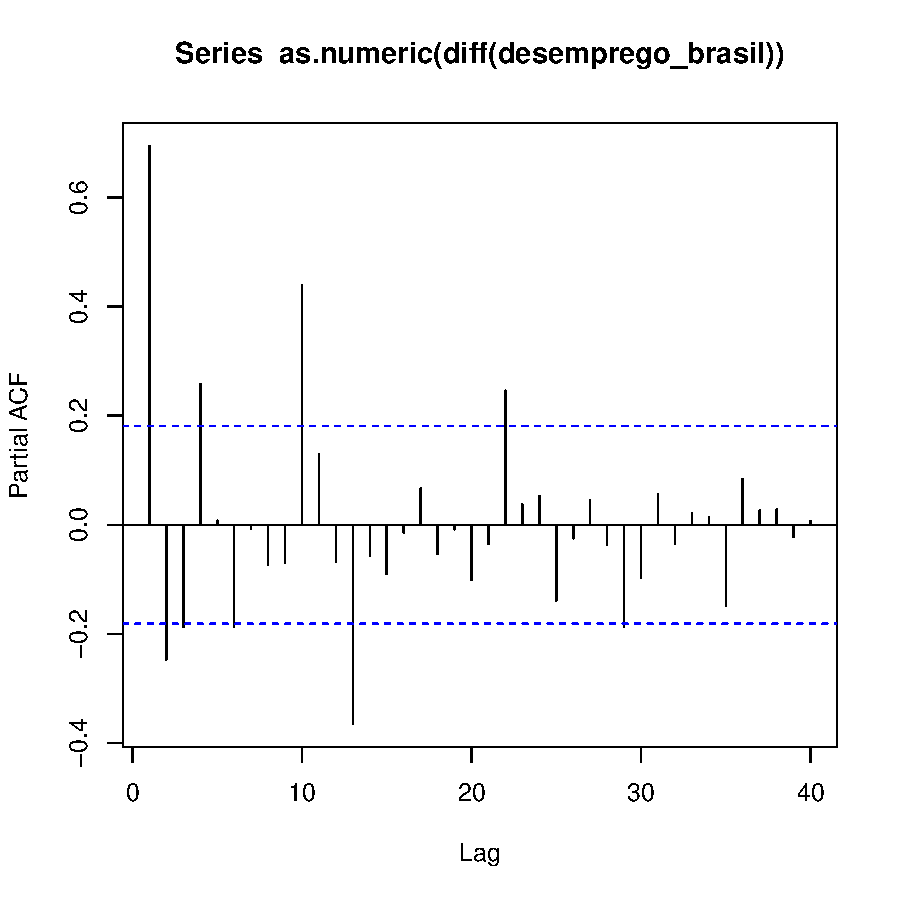
\includegraphics[scale=0.39]{graficos/pacf_unemp.pdf}
	\end{figure}
\end{frame}

\begin{frame}{Inferência conjunta sobre a FAC}
	\begin{itemize}
	 	\item Para testar a nula conjunta de que $\gamma_{1} = \gamma_{2}=\ldots = \gamma_{s} = 0$, onde $s$ é pequeno relativamente a $T$, podemos usar a {\color{blue}estatística de Ljung-Box}:
		
		$$\hat{Q}= T(T+2)\sum_{r=1}^s \frac{\hat{\gamma}_r^2}{T-k}\, .$$
		\item Com $T$ grande, sob a nula, $\hat{Q}$ segue uma qui-quadrado com $s$ graus de liberdade. Valores altos da estatística são evidência contra a nula, i.e. evidência de que ao menos uma autocorrelação entre as testadas é diferente de zero.
	\end{itemize}
\end{frame}



\begin{frame}{FAC e FACP de um AR(p) estacionário}
	\begin{halfwideitemize}
		\item Como vimos em aula anterior, a FAC de um AR(1) estacionário é dada por:
		\begin{equation}
			\gamma_k = \text{cor}(Y_t, Y_{t-k}) = \beta_1^k, \quad |\beta_1| < 1
		\end{equation}
		isto é, a FAC apresenta decaimento geométrico em direção a zero.
		\item De modo geral, a FAC de um AR(p) estacionário apresenta {\color{blue}decaimento em direção a zero}, visto que um AR(p) estacionário pode ser escrito como um MA($\infty$), i.e.
		\begin{equation}
			Y_t = \mu + \epsilon_t + \sum_{j=1}^\infty  \omega_j \epsilon_{t- j}
		\end{equation}
		\item E a FACP de um AR(p) estacionário? Pela definição da FACP de ordem $k$ como o coeficiente de $Y_{t-k}$ na regressão populacional de $Y_t$ em $Y_{t-1}$, $Y_{t-2}$,\ldots $Y_{t-k}$, esperamos que a FACP seja {\color{blue} truncada em $p$}, visto que o processo só depende diretamente das $p$ primeiras defasagens.
	\end{halfwideitemize}
\end{frame}
\begin{frame}{Exemplo: FAC e FACP estimadas de um AR(2) (T=10.000)}
	\begin{figure}
		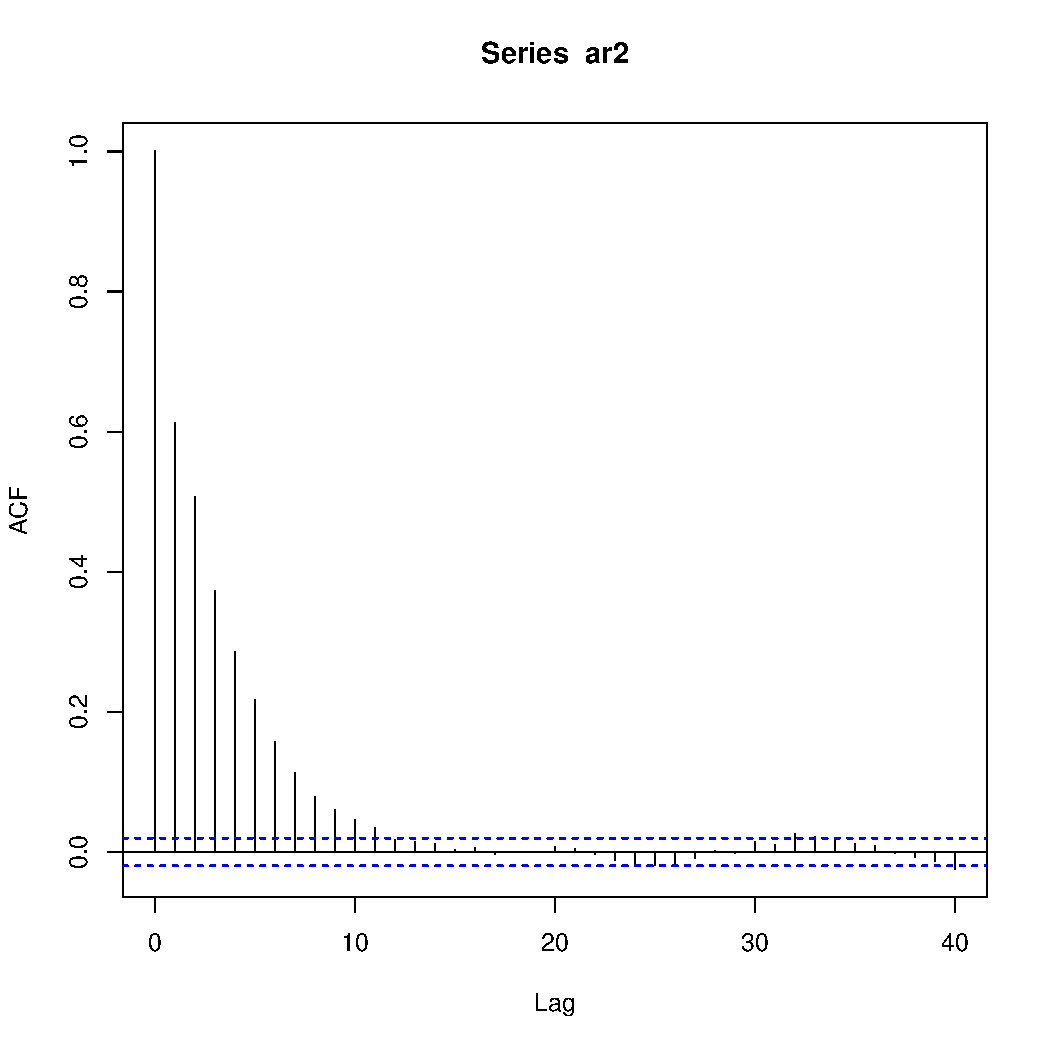
\includegraphics[scale=0.33]{graficos/ar2_fac.pdf} 		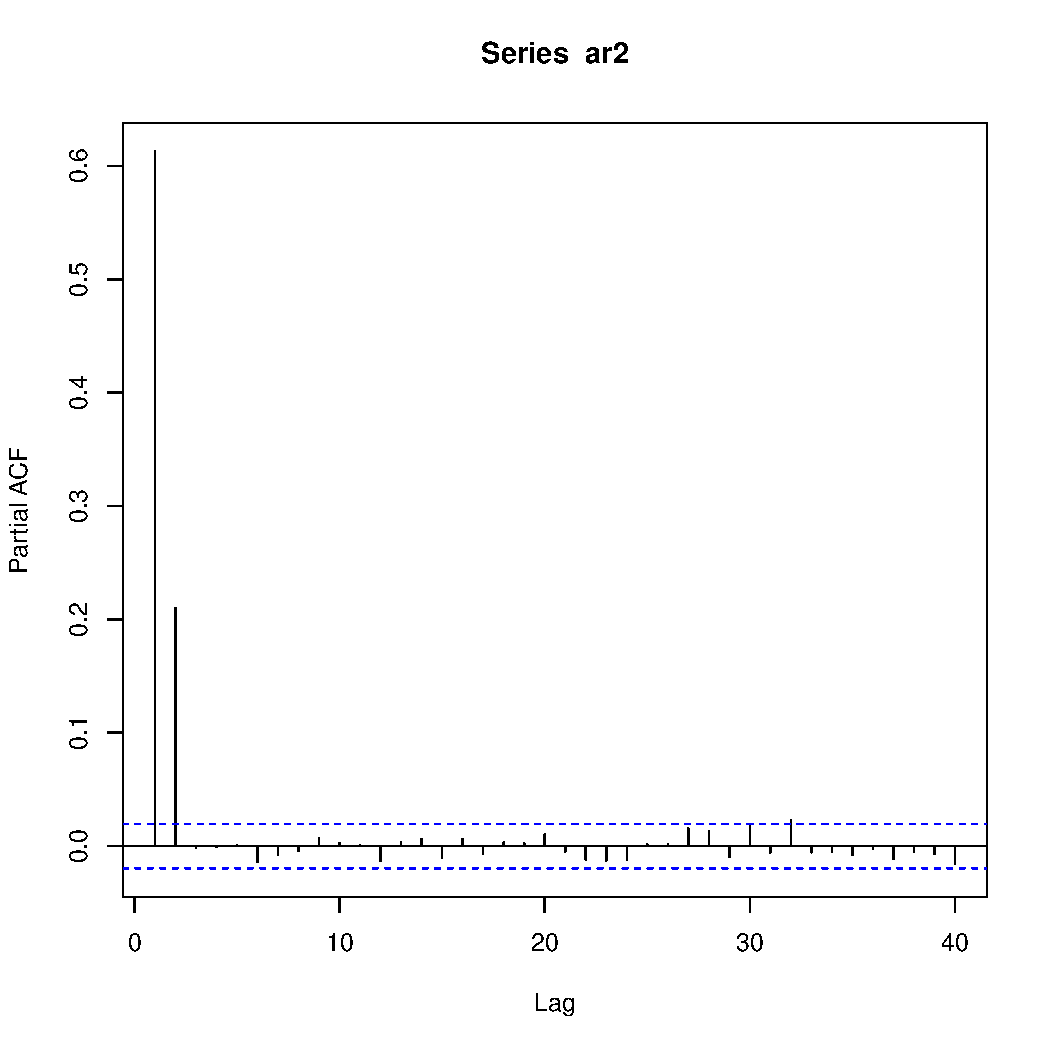
\includegraphics[scale=0.33]{graficos/ar2_facp.pdf}
	\end{figure}
\end{frame}
\begin{frame}{FAC e FACP de um MA(q) invertível}
	\begin{halfwideitemize}
		\item Como vimos em aula anterior, a FAC de um MA(q) é {\color{blue}truncada} em $q$, visto que a correlação morre após $q$ períodos.
		\item E a FACP? Se o processo MA for invertível, vimos que ele pode ser escrito como um $AR(\infty)$. Dessa representação, fica claro que a FACP de um MA(q) apresenta {\color{blue}decaimento em direção a zero}. 
	\end{halfwideitemize}
\end{frame}
\begin{frame}{Exemplo: FAC e FACP estimadas de um MA(3) (T=10.000)}
	\begin{figure}
		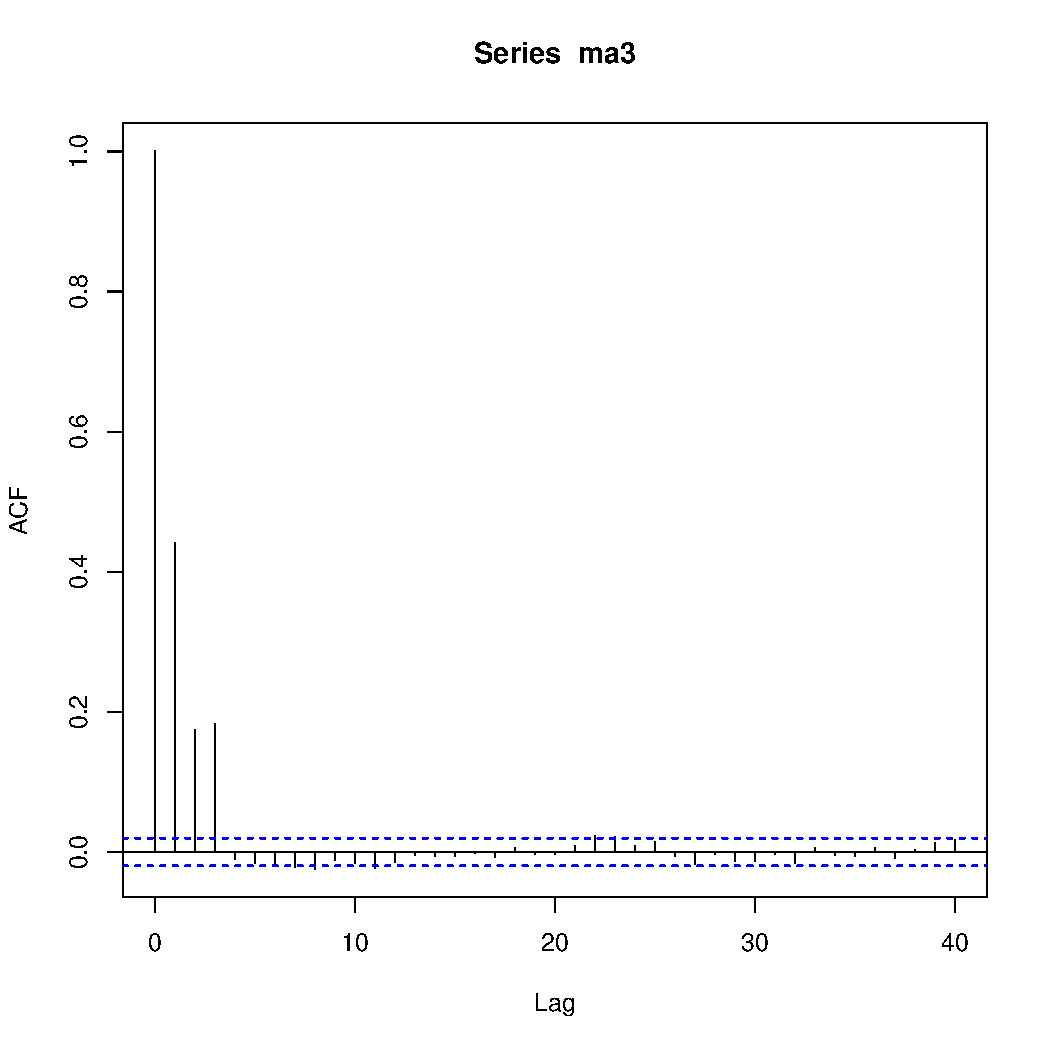
\includegraphics[scale=0.33]{graficos/ma3_fac.pdf} 		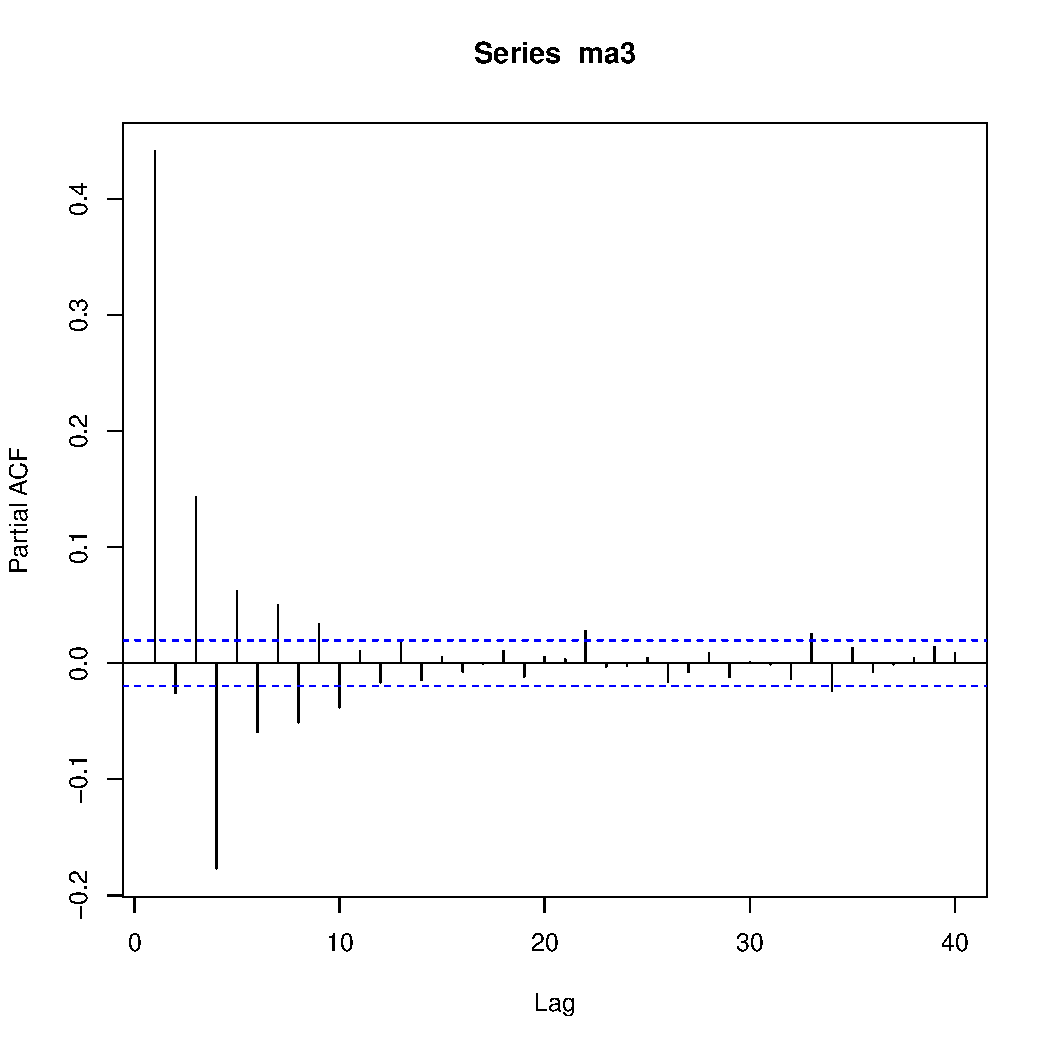
\includegraphics[scale=0.33]{graficos/ma3_facp.pdf}
	\end{figure}
\end{frame}

\begin{frame}{FAC e FACP de um ARMA(p,q) estacionário e invertível}
	\begin{halfwideitemize}
		\item Generalizando a discussão anterior, um ARMA(p,q) estacionário cuja parte MA é invertível pode ser representado tanto como um $AR(\infty)$ como um $MA(\infty)$. Nesse caso, {\color{blue}tanto a FAC como a FACP apresentam decaimento}.
		\item Nesses casos, costuma-se considerar a ordem máxima $q_{\text{max}}$ em que a FAC torna-se pouco significativa e a ordem $p_{\text{max}}$ em que a FACP torna-se pouco signifcativa e considerar todos os ARMA(p,q), $0 \leq p\leq p_{\text{max}}$ e $0 \leq q \leq q_{\text{max}}$ como candidatos.
	\end{halfwideitemize}
\end{frame}

\begin{frame}{Exemplo: FAC e FACP estimadas de um ARMA(2,3) (T=10.000)}
	\begin{figure}
		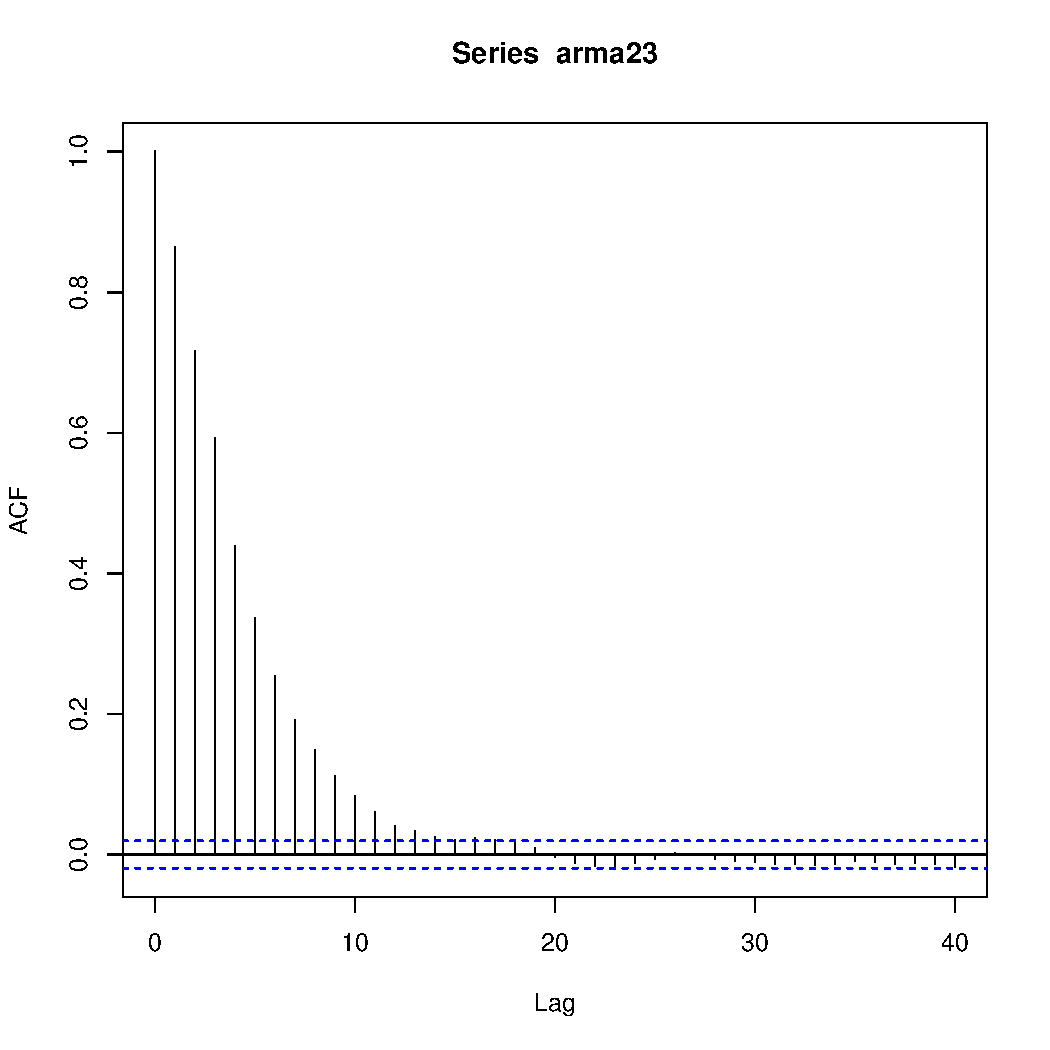
\includegraphics[scale=0.33]{graficos/arma23_fac.pdf} 		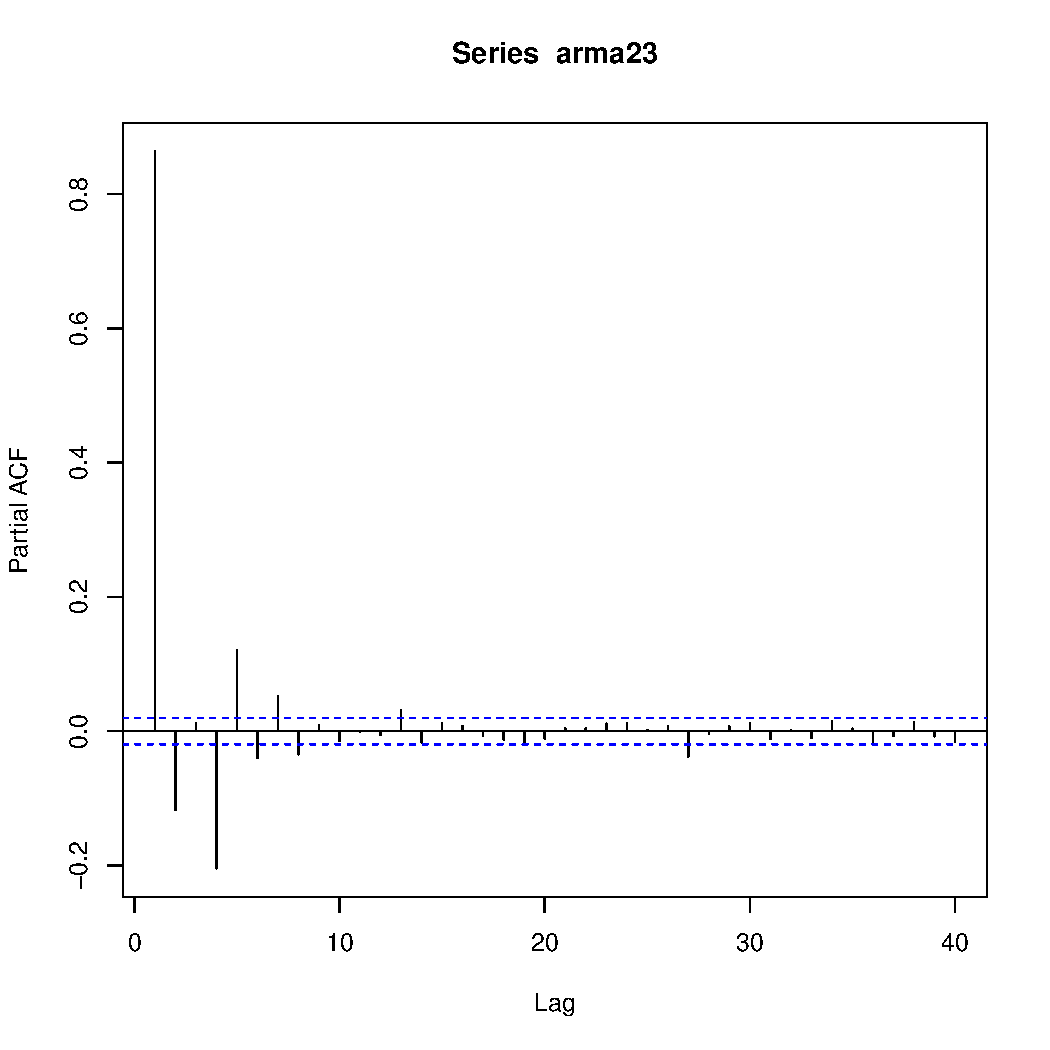
\includegraphics[scale=0.33]{graficos/arma23_facp.pdf}
	\end{figure}
\end{frame}
\begin{frame}{Resumo}
	\begin{table}[H]
		\begin{center}
			\begin{tabular}{c|c|c}
				
				Modelo& FAC & FACP   \\
				\hline
				AR(p) estacionário& decai  & truncada em $p$  \\
				\hline
				MA(q) invertível& truncada em $q$ & decai   \\
				\hline
				ARMA(p,q) estacionário  & decai  & decai  \\
				e invertível& (esp. após $q$) & (esp. após $p$)
			\end{tabular}
		\end{center}
	\end{table}
\end{frame}

\end{document}